\documentclass[dvipsnames]{beamer}
\input{mybeamerdefs}

\begin{document}

\begin{frame}{\today}
\begin{itemize}
\item I looked into the distortion from the metabolic image of 2019-12-12 based on the BW per pixel and frequency offset between metabolites.
\end{itemize}
\end{frame}

\section{Distortion from metabolic image}

\begin{frame}{Summary}
\begin{itemize}
\item I found the BW per pixel to be 125 Hz.
\item I found the frequency offset to be -1277 Hz.
\item \begin{equation*} \mathrm{int}\left(\frac{-1277 Hz}{125 Hz} \right) = -10\end{equation*}
\item Take a look at the image.
\end{itemize}
\end{frame}

\begin{frame}{Image from 2019-12-12}
\begin{center}
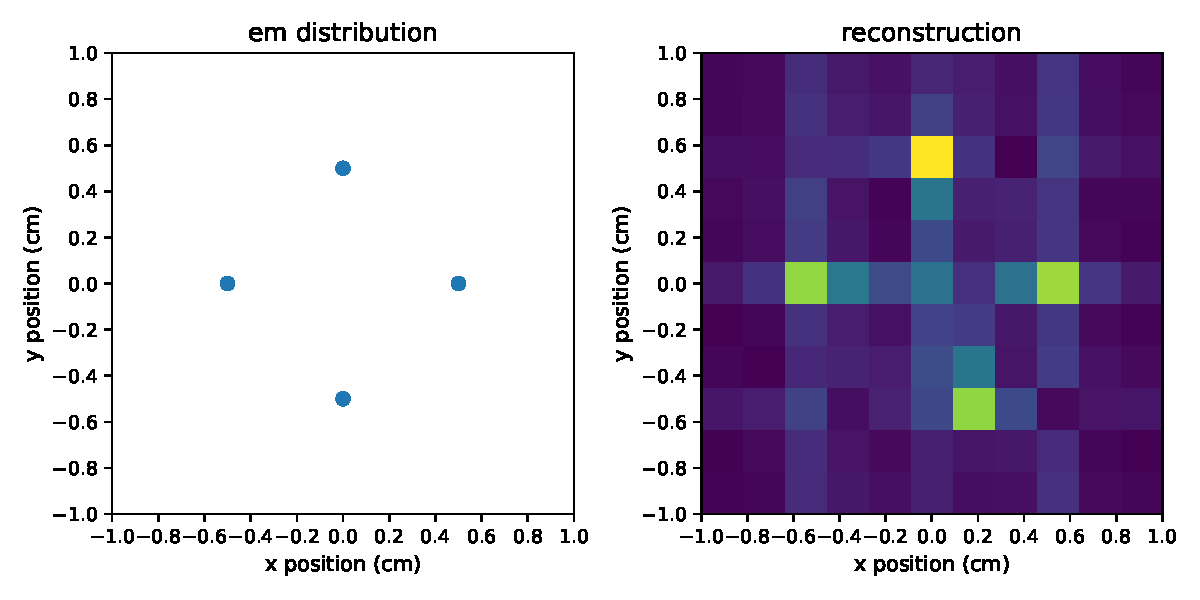
\includegraphics[width=\textwidth]{reconstruction_metabolism-on-20percent}
\end{center}
\end{frame}

\begin{frame}{Comments}
\begin{itemize}
\item The bottommost em is shifted 10 pixels to the left (if you wrap around to the other side of the image). Checks out!
\end{itemize}
\end{frame}

\end{document}